% 第6章第2节：图拉普拉斯（邻域汇总、组合拉普拉斯、二次型与沿边变化能量）。

\section{图拉普拉斯}
\label{sec:graph-laplacian}

上一节得到了每条边上的差，但还没有把它们组织成作用于顶点函数的算子。本节沿两条路线构造同一个算子：一条在每个顶点读取邻居并与本点比较，另一条先取边差、再按边权缩放、最后汇总回顶点。两条路线的结果都是组合拉普拉斯，它的二次型累计各边差值的平方，用来衡量函数沿边变化的总量。

\subsection{邻域汇总}
\label{sec:graph-spec-neighborhood-aggregation}

最直接的图上运算是读取邻居。用权矩阵$\bm W$左乘顶点函数，
\[
 (\bm W\bm f)_i=\sum_{j=1}^nw_{i,j}f_j ,
\]
第$i$个输出把各邻居的值按边权加权求和；非邻居的$w_{i,j}=0$，不参与计算。与之相伴的量是顶点$i$的\term{加权度}（weighted degree）
\[
 d_i=\sum_{j=1}^nw_{i,j},\qquad \bm D=\operatorname{diag}(d_1,\ldots,d_n),
\]
它累计与$i$相连的全部边权。第~\ref{sec:graph-adjacency-paths}节的度数的是邻居个数，加权度数的是连接强度，只有每条边权都为$1$时二者才相等。本章后文所说的度一律指加权度。

$\bm W\bm f$是加权和，不是平均。在单位权三点路径上取$\bm f=(3,1,2)^{\top}$，得到$\bm W\bm f=(1,5,1)^{\top}$：中间顶点读到两个邻居之和$5$，比任何一个邻居的值都大。要得到邻居的平均，还须除以加权度，这是第~\ref{sec:graph-normalized-laplacian}节的工作。

\paragraph{同步读取与就地更新}
“作用一次”还有一个容易忽略的约定：所有顶点都从同一份旧向量读取，结果写入另一份新数组。若在原数组上就地按编号逐个更新，后更新的顶点会读到本轮已经改写的值。在上面的例子中按$1,2,3$的次序就地更新：先得$v_1=f_2=1$；更新顶点$2$时读到的是新值$v_1=1$而不是$3$，得$v_2=1+2=3$；再得$v_3=v_2=3$。结果是$(1,3,3)^{\top}$而不是$(1,5,1)^{\top}$。就地更新实现的是另一个与次序有关的映射，不再是$\bm W$。本章所说的算子作用都指同步读取旧值，只涉及一次线性映射，不涉及随时间演化的过程。

\subsection{组合拉普拉斯}
\label{sec:graph-spec-combinatorial-laplacian}

邻域汇总给出了邻居的加权和，衡量变化还需要把本点值与邻居值相比较。对每个邻居取差$f_i-f_j$，再按边权求和，得到
\[
 \sum_{j=1}^nw_{i,j}(f_i-f_j)=d_if_i-(\bm W\bm f)_i .
\]
右端对每个$i$成立，于是这一运算可以写成矩阵$\bm D-\bm W$。

\begin{definition}[组合拉普拉斯]
\label{def:graph-spec-combinatorial-laplacian}
设$\mathcal G=(V,E)$为有限无向图，边权对称非负、无自环，$\bm W$与$\bm D$分别为权矩阵与加权度矩阵。称
\begin{equation}
 \bm L=\bm D-\bm W
 \label{eq:graph-spec-laplacian}
\end{equation}
为$\mathcal G$的\term{组合图拉普拉斯}（combinatorial graph Laplacian），它逐点作用为$(\bm L\bm f)_i=\sum_jw_{i,j}(f_i-f_j)$。
\end{definition}

逐项看，$\bm L$的对角元是加权度$d_i$，非对角元是$-w_{i,j}$；每行之和为$d_i-\sum_jw_{i,j}=0$，所以$\bm L\bm1=\bm0$，常量函数被映成零。这与直觉一致：常量在每条边上都没有差。单位权三点路径的拉普拉斯为
\[
 \bm L=\begin{bmatrix}1&-1&0\\-1&2&-1\\0&-1&1\end{bmatrix},\qquad
 \bm L\begin{bmatrix}3\\1\\2\end{bmatrix}=\begin{bmatrix}2\\-3\\1\end{bmatrix}.
\]
中间顶点的输出$-3$是它与两个邻居之差的和$(1-3)+(1-2)$，负号表示它比邻居低。

\begin{figure}[!htb]
  \centering
  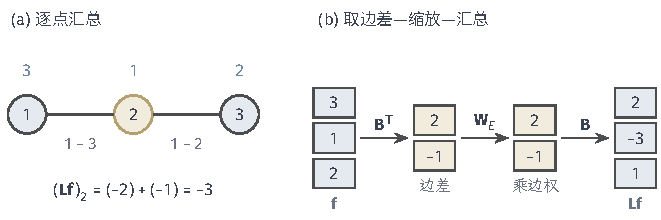
\includegraphics[width=112mm]{figures/01-basic-mathematics/04-graphs/tikz/c6-laplacian-two-routes/figure.pdf}
  \caption{同一个拉普拉斯的两条计算路线，单位权三点路径，$\bm f=(3,1,2)^{\top}$。(a)~在黄色顶点$2$处把本点值与每个邻居值相减再求和，得$(\bm L\bm f)_2=-3$；(b)~先用$\bm B^{\top}$取边差$(2,-1)$，再乘边权（此处均为$1$），最后用$\bm B$按净流出汇总回顶点，得到完整的$\bm L\bm f=(2,-3,1)^{\top}$。两条路线在每个顶点给出相同结果。}
  \label{fig:graph-spec-laplacian-two-routes}
\end{figure}

\paragraph{取边差、缩放、汇总}
第二条路线把上一节的边差接进来：先用$\bm B^{\top}$取边差，再用$\bm W_E$把第$e$条边的差乘以$w_e$，最后用$\bm B$按净流出汇总回顶点。三步合起来是矩阵$\bm B\bm W_E\bm B^{\top}$。为了核对它等于$\bm L$，记$\bm b_e$为$\bm B$的第$e$列，则
\[
 \bm B\bm W_E\bm B^{\top}=\sum_{e\in E}w_e\bm b_e\bm b_e^{\top}.
\]
若$e$连接$i$与$j$，则$\bm b_e=\pm(\bm e_i-\bm e_j)$，$\bm b_e\bm b_e^{\top}$在$(i,i)$、$(j,j)$处为$1$，在$(i,j)$、$(j,i)$处为$-1$，其余为零，而且与参考方向无关。逐边相加，每个对角位置累计出$d_i$，每个非对角位置得到$-w_{i,j}$，因此
\begin{equation}
 \bm L=\bm B\bm W_E\bm B^{\top}.
 \label{eq:graph-spec-laplacian-incidence}
\end{equation}
图~\ref{fig:graph-spec-laplacian-two-routes}在三点路径上并排执行了两条路线。

\paragraph{与参考方向无关}
上一节要求无向图算子不依赖参考方向，式~\eqref{eq:graph-spec-laplacian-incidence}可以整体核对这一点。改记部分边的方向后，关联矩阵变为$\bm B\bm R$，其中$\bm R$是对角元为$\pm1$的符号矩阵。由于对角矩阵相乘可以交换、$\bm R^2=\bm I$，有$\bm R\bm W_E\bm R=\bm W_E$，于是
\[
 (\bm B\bm R)\bm W_E(\bm B\bm R)^{\top}=\bm B\bm R\bm W_E\bm R\bm B^{\top}=\bm B\bm W_E\bm B^{\top}.
\]
边差变号了两次，一次在取差时，一次在汇总时，两次抵消。这一抵消依赖于参考方向只是记账约定；对真正的有向图，弧的方向是数据本身，不能用同样的理由消去，有向图的拉普拉斯一般不对称，不在本章范围内。

\subsection{二次型与沿边变化能量}
\label{sec:graph-spec-dirichlet-energy}

有了算子，再看它的二次型能说明什么。把式~\eqref{eq:graph-spec-laplacian-incidence}代入$\bm f^{\top}\bm L\bm f$，中间恰好是边差的加权平方和：
\begin{equation}
 \begin{aligned}
 \bm f^{\top}\bm L\bm f
 &=(\bm B^{\top}\bm f)^{\top}\bm W_E(\bm B^{\top}\bm f)
 =\sum_{\{i,j\}\in E}w_{i,j}(f_i-f_j)^2\\
 &=\frac12\sum_{i=1}^n\sum_{j=1}^nw_{i,j}(f_i-f_j)^2 .
 \end{aligned}
 \label{eq:graph-spec-dirichlet-energy}
\end{equation}
中间的和对无向边求和，每条边计一次；最右端对有序点对$(i,j)$求和，每条边作为$(i,j)$与$(j,i)$各出现一次，所以要乘$\frac12$。这个量称为沿边变化能量，也称\term{Dirichlet能量}（Dirichlet energy）。它的大小取决于两样东西：相邻值差多少，以及图要求这一对顶点被比较得多强。

\begin{figure}[!htb]
  \centering
  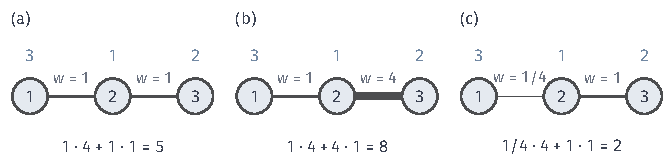
\includegraphics[width=112mm]{figures/01-basic-mathematics/04-graphs/tikz/c6-energy-edge-weights/figure.pdf}
  \caption{同一顶点函数$\bm f=(3,1,2)^{\top}$在三组边权下的沿边变化能量，线宽示意边权大小。两条边的差的平方始终为$4$与$1$，能量是它们的加权和：(a)~权$(1,1)$时为$5$；(b)~加重边$\{2,3\}$后为$8$；(c)~减轻边$\{1,2\}$后为$2$。}
  \label{fig:graph-spec-energy-edge-weights}
\end{figure}

图~\ref{fig:graph-spec-energy-edge-weights}固定$\bm f=(3,1,2)^{\top}$，只改变边权。两条边的差的平方始终是$4$和$1$。单位权时能量为$4+1=5$；把$\{2,3\}$的权加到$4$，较小的差被放大四倍，能量变为$4+4=8$；把$\{1,2\}$的权减到$\frac14$，较大的差几乎不再计入，能量降到$1+1=2$。所以说一个函数“平滑”，总是相对于给定的边权而言的。

\paragraph{半正定与零能量}
式~\eqref{eq:graph-spec-dirichlet-energy}的每一项都是非负权乘平方，所以对任意$\bm f$都有$\bm f^{\top}\bm L\bm f\geq0$。$\bm L$又是对称矩阵，因此它对称半正定（第~\ref{sec:ls-gram-psd}节）。这一结论用到了权非负：若允许负权，对应的项可以为负，半正定性一般不再成立。

能量何时为零？各项非负，总和为零当且仅当每一项为零，即对每条正权边都有$f_i=f_j$；零权边的项本来就是零，不对两端施加任何限制。这是逐边的条件。相等关系怎样沿正权路径传递，零能量的函数究竟有哪些，要用到连通分量，留到第~\ref{sec:graph-spectrum-connectivity}节统一回答。
